
\documentclass[oneside,12pt]{book}

\usepackage[utf8]{inputenc}
\usepackage[greek, english]{babel}

% Packages
\usepackage{alphabeta}
\usepackage{amsmath}
\usepackage{amsthm}
\usepackage{caption}
\usepackage{color}
\usepackage{fullpage}
\usepackage{graphicx}
\usepackage{latexsym}
\usepackage{listings}
\usepackage{pxfonts}
\usepackage{stackrel}
\usepackage{titlesec}
\usepackage{subfig}
\usepackage{tikz}
\usepackage{float}
\usepackage{hyperref}
\usepackage{setspace}
\usepackage{tcolorbox}
\usepackage[ruled,vlined]{algorithm2e}
\tcbuselibrary{theorems}

\addto{\captionsenglish}{\renewcommand{\bibname}{}}
\patchcmd{\thebibliography}{\chapter*}{\section*}{}{}

\newtcbtheorem[number within=section]{mytheorem}{Ορισμός}%
{colback=black!5,colframe=black!15!black,fonttitle=\bfseries}{th}

\newtcbtheorem[number within=section]{theorem}{Θεώρημα}%
{colback=black!5,colframe=black!15!black,fonttitle=\bfseries}{th}

% Commands
\newcommand{\N}{\mathbb{N}}
\newcommand{\R}{\mathbb{R}}
\newcommand{\code}[2]{\lstinputlisting[caption={#2}]{#1}}
\newcommand{\margin}{\hspace{4pt}}
\newcommand{\norm}[1]{\left\lVert#1\right\rVert}
\newcommand{\abs}[1]{\left\lvert#1\right\rvert}

% Environments
\newenvironment{matlab}
	{\begin{figure}[hp]\centering\captionsetup{justification=centering}}
	{\end{figure}}

\newenvironment{rcases}
	{\left.\begin{aligned}}
	{\end{aligned}\right\rbrace}
% Python Syntax Highlighting
\definecolor{string_color}{RGB}{0, 161, 13}
\definecolor{comment_color}{RGB}{46, 46, 46}
\definecolor{keyword_color}{RGB}{0, 112, 191}
\definecolor{background_color}{RGB}{250, 250, 250}
\lstset{
    framesep=15pt,
    xleftmargin=15pt,
    xrightmargin=15pt,
    language=Python,
    captionpos=b,
    numbers=right,
    numberstyle=\small\ttfamily,
    frame=lines,
    showspaces=false,
    showtabs=false,
    breaklines=true,
    showstringspaces=false,
    breakatwhitespace=true,
    commentstyle=\color{comment_color}\textit,
    keywordstyle=\bfseries\color{keyword_color}\textbf,
    stringstyle=\color{string_color}\textit,
    morekeywords={self, lambda, __init__, __del__, __name__, for, in, not, and, or, :},
    basicstyle=\small\ttfamily,
    tabsize=4,
    keepspaces=true,
    columns=flexible,
    backgroundcolor=\color{background_color}
}
% Links
\hypersetup{
    colorlinks=true,
    linkcolor=blue,
    filecolor=magenta,
    urlcolor=cyan,
}
% Lengths
\setlength{\parindent}{0in}
\setlength{\oddsidemargin}{0in}
\setlength{\textwidth}{6.5in}
\setlength{\textheight}{10in}
\setlength{\topmargin}{-1.0in}
\setlength{\headheight}{18pt}
\setlength{\parskip}{0.3cm}
\setlength{\parindent}{5ex}
\doublespacing
\theoremstyle{definition}
\newtheorem{definition}{Definition}[section]
\titlespacing*{\subsection}
{0pt}{5.5ex plus 1ex minus .2ex}{4.3ex plus .2ex}
\title{\huge Travelling Salesman Problem}
\author{Σιώρος Βασίλειος\\Ανδρινοπούλου Χριστίνα}
\date{Μάϊος 2020}
\begin{document}
\maketitle
\pagenumbering{gobble}
\pagebreak
\tableofcontents

\chapter{Abstract}

\chapter{Introduction}

Το "Travelling Salesman Problem" (TSP) ή με την ελληνική του απόδοση "Πρόβλημα του πλανόδιου πωλητή" (ή εναλλακτικά πρόβλημα του περιοδεύοντος πωλητή) είναι ένα κλασσικό πρόβλημα θεωρητικής επιστήμης των  υπολογιστών. Πρόκειται για ένα πρόβλημα περιήγησης. Ο πωλητής οφείλει να επισκευτεί n το πλήθος πόλεις για να πουλήσει το εμπόρευμά του. Σκοπός του προβλήματος είναι η εύρεση μίας βέλτιστης διαδρομής για τον πωλητή, με την οποία θα μπορέσει να επισκεφτεί όλες τις πόλεις που τον ενδιαφέρουν, μόνο μία φορά την κάθε μία και μάλιστα με τέτοιον τρόπο ώστε να διανύσει τη μικρότερη δυνατή απόσταση. Με άλλα λόγια, ο πωλητής πρέπει να επισκεφτεί την κάθε πόλη ακριβώς μία φορά ακολουθώντας το συντομότερο δρομολόγιο. \\

Το πρόβλημα του περιοδεύοντος πωλητή έχει αποδειχθεί ότι είναι NP-hard (NP-δύσκολο), έννοια την οποία θα αναλύσουμε παρακάτω. Ωστόσο, έχουν γίνει σημαντικές προσπάθειες από την επιστημονική κοινότητα, ώστε οι αλγόριθμοι TSP να βελτιωθούν αισθητά ως προς τις αποδόσεις τους. \\

Φυσικά, το TSP είναι ένα πολύ σημαντικό πρόβλημα στην επιστήμη της πληροφορικής, καθώς έχει μία γκάμα εφαρμογών. Τέτοιες είναι: ο σχεδιασμός των μετακινήσεων των συσκευων αυτόματης διατήρησης καρτών ηλεκτρονικών κυκλωμάτων, οι μηχανές εφοδιασμού στους ορόφους καταστημάτων ή σε αποθήκες κ.α. 

\begin{matlab}
	
\includegraphics[scale=0.8]{images/tsp.png}
	\caption{Travelling Salesman Problem - TSP \\ πηγή: https://www.localsolver.com/docs/last/exampletour/tsp.html1}
\end{matlab}

\chapter{Μαθηματικό υπόβαθρο}

Η μελέτη σε βάθος του προβλήματος του περιοδεύοντος πωλητή χρήζει απαραίτητη την γνώση μερικών βασικών μαθηματικών εννοιών. Στο κεφάλαιο αυτό, παρουσιάζουμε και αναλύυμε, στον βαθμό που κρίνεται απαραίτητο, όλες τις μαθηματικές γνώσεις που χρειάζονται για την κατανοήση του TSP. \\

\section{Γραφήματα}

Βασική έννοια για τη μελέτη του προβήματος του περιοδέυοντος πωλητή είναι τα γραφήματα. Τα γραφήματα είναι ένα πολύ σημαντικά εργαλείο στα χερια των θεωρητικών πληροφορικών. Προσφέρουν πολλές διευκολύνσεις κατά τη μελέτη προβλημάτων (όπως και στην περίπτωση μας), είναι σχετικά απλά στη μελέτη και την κατανόηση τους και μπορούν εύκολα να κωδικοποιηθούν και να θεμελιωθούν με αυστηρό, μαθηματικό τρόπο. \\

\subsection{Βασική ορολογία}

Τα βασικά συστατικά ενός γραφήματος είναι  οι κορυφές και οι ακμές. Οι κορυφές ενώνονται με τη βοήθεια των ακμών και δημιουργούν ένα γράφημα. \\

Τα γραφήματα μπορούν να διακριθούν σε δύο βασικές κατηγορίες, τα κατευθυνόμενα γραφήματα και τη μη κατευθυνόμενα. \\

Ο αφηρημένος ορισμός στην περίπτωση των κατευθυνόμενων γραφημάτων περιλαμβάνει ένα διατεταγμένο ζεύγος \((V,E)\), όπου \(V\) είναι το σύνολο και το \(E\) είναι μία διμελής σχέση. Το \(V\) αποτελεί το σύνολο των κορυφών και το \(E\) το σύνολο των ακμών. Το κατευθυνόμενο γράφημα συμβολίζεται με \(G\). Ένα κατευθυνόμενο γράφημα μπορεί να αναπαρασταθεί γεωμετρικά ως ένα σύνολο από \(V\) σημεία, τα οποία ενώνονται με \(E\) βέλη. Ενα παραδειγμα γράφου φαίνεται στην εικόνα παρακάτω.

\begin{matlab}
	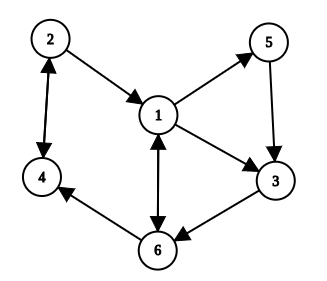
\includegraphics[scale=0.8]{images/directed_graph_example.png}
	\caption{Παράδειγμα κατευθυνόμενου γράφου \\ κατασκευάστηκε με: https://csacademy.com/app/graph\_editor/}
\end{matlab} 

Ο ορισμός για το μη κατευθυνόμενο γράφημα περιλαμβάνει ένα σύνολο \(V\) και ένα σύνολο πολυσυνόλων δύο στοιχείων \(E\). Το \(V\) αποτελεί και σε αυτήν την περιπτωση το σύνολο των κορυφών και το \(E\) το σύνολο των ακμών. Μία ενδεικτική γεμετρική αναπαράσταση δίνεται στην αντίστοιχη εικόνα παρακάτω. Και σε αυτήν την περίπτωση το \(V\) είναι ένα σύνολο σημείων, ωστόσο το \(E\) είναι ένα σύνολο γραμμών που δεν υποδικνύουν καμμία κατεύθυνση. \\

\begin{matlab}
	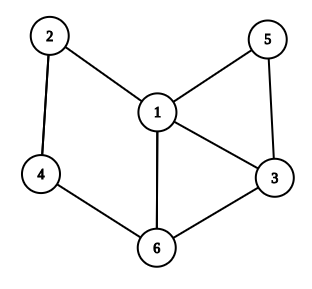
\includegraphics[scale=0.8]{images/undirected_graph_example.png}
	\caption{Παράδειγμα μη κατευθυνόμενου γράφου \\ κατασκευάστηκε με: https://csacademy.com/app/graph\_editor/}
\end{matlab}   

\subsection{Μονοπάτια}

Σε κάθε κατευθυνόμενο γράφημα οι ακμές περιέχουν μία αρχική κορυφή και μία τερματική κορυφή. Για παράδειγμα η ακμή (1,3) της εικόνας 3.1 περιέχει δύο κορυφές. Η κορυφή 1 καλείται αρχική κορυφή και η κορυφή 3 καλείται τερματική κορυφή. \\

Στα κατευθυνόμενα γραφήματα, μία ακολουθία ακμών \((e_1, e_2,...,e_k)\) όπου η τερματική κορυφή μίας ακμής \(e_j\) ταυτίζεται με την αρχική κορυφή της \(e_{(j+1)}\) καλείται μονοπάτι. \\

Αν ένα μονοπάτι δεν περιέχει την ίδια ακμή δύο φορές ονομάζεται απλό μονοπάτι. \\

Στοιχειώδες μονοποάτι καλείται το μονοπάτι εκείνο όπου δεν περιέχει την ίδια κορυφή παραπάνω από μία φορά. \\

Κύκλωμα καλείται το μονοπάτι \((e_1, e_2,...,e_k)\), όπου η τερματική κορυφή της \(e_k\) ακμής συμπίπτει με την αρχική κορυφή της \(e_1\) ακμής. \\

\subsection{Χαμιλτόνειοι κύκλοι και μονοπατια}

O Ιρλανδός φυσικός και μαθηματικός William Rowan Hamilton (4 Αυγούστου 1805 – 2 Σεπτεμβρίου 1865) μελέτησε εκτός των άλλων και τα γραφήματα. Συγκεκριμένα, δημιούργησε το μαθηματικό παιχνίδι "ο γύρος του κόσμου", του οποίου σκοπός ήταν η εύρεση ενός μονοπατιού από ακμές δωδεκαέδρου. Το μονοπάτι έπρεπε να περνά από κάθε κορυφή του δωδεκαέδρου ακριβώς μία φορά. Πιο συγκεκριμένα, ο ένας παίκτης κάρφωνε από μία βελόνα σε 5 διαδοχικές κορυφές και έπειτα ο άλλος παίκτης έπρεπε να συμπληρώσει το κύκλωμα έτσι ώστε να περιλαμβάνει όλες τις κορυφές. Μάλιστα, σε επιστολή προς τον φίλο του John T. Graves (17 Οκτωβρίου 1856) ο Hamilton τον πληροφορεί σχετικά με ένα παιχνίδι που βασίζεται στον εικοσιανό λογισμό (αλγεβρική δομή για τον υπολογισμών συμμετριών του εικοσαέδρου από τον ίδιο τον Hamilton) και την αναγνωρισιμότητα που έχει λάβει από μερικούς νεαρούς. Το παιχνίδι αυτό στάθηκε η αφορμή για την ανάπτυξη της θεωρίας γύρω από τα γραφήματα και προς τιμήν του Hamilton και του εν λόγω παιχνιδιού που επινόησε οι Χαμιλτονειανοί κύκλοι έλαβαν το όνομά του. \\

\begin{matlab}
	\includegraphics[scale=0.2]{images/Hamilton.png}
	\caption{William Rowan Hamilton \\ πηγή: https://en.wikipedia.org/wiki/William\_Rowan\_Hamilton}
\end{matlab}  

Η εύρεση ενός μονοπατιού ή ενός κυκλώματος που περνά από κάθε κορυφή ενός δεδομένου γραφήματος μόνο μία φορά φαντάζει αρχικά απλή υπόθεση, ωστόσο οι μέχρις στιγμής επιστημονικές προσεγγίσεις αποδεκνύουν το αντίθετο. 

Μονοπάτι (ή κύκλωμα) Hamilton είναι ένα μονοπάτι (ή ένα κύκλωμα) που περνά από όλες τις κορυφές ενός γραφήματος ακριβώς μία φορά. \\

Ένα γράφημα που περιέχει κύκλο Hamilton καλείται χαμιλτόνειο, ενώ αν δεν περιέχει καλείται μη χαμιλτόνειο. \\

Δυστυχώς, μέχρι και τώρα δε γνωρίζουμε κάποια ικανή και αναγκάια συνθήκη για την ύπαρξη μονοπατιών και κυκλωμάτων Hamilton. Δοθέντος ενός γραφήματος G, η απόδειξη ύπαρξης ή μη ενός μονοπατιού ή κυκλώματος Hamilton είναι η κατασκευή του. \\ 

\chapter{Γραφοθεωρητική Προσέγγιση του Προβλήματος του πλανόδιου πωλητή}
 
Η προσέγγιση του TSP με βάση τη θεωρία γραφημάτων συνδέεται στενά με τα τους Χαμιλτόνειους κύκλους. Επί της ουσίας το πρόβλημα του περιοδεύονοτς πωλητή είναι μία επέκταση του προβλήματος εύρεσης κυκλώματος Hamilton. \\ 

Όπως ήδη έχουμε αναφέρει στην εισαγωγή, στόχος του προβλήματος είναι ο πωλητής να επισκεφτεί ένα σύνολο πόλεων, ακριβώς μία φορά την κάθε μία, ελαχιστοποιόντας τις αποστάσεις που πρέπει να διανύσει. Αν αναπαραστήσουμε το σύνολο των πόλεων προς επίσκεψη με ένα σύνολο κορυφών \(V\) και το σύνολο όλων των πιθανών διαδρομών με ενα σύνολο \(E\), τότε μπορούμε να μεταφέρουμε την εικόνα του χάρτη που μελετά ο πωλητής σε γραφική αναπαράσταση. Ο πωλητής εκκινεί και τερματίζει το ταξίδι του στην ίδια πόλη και επισκέπτεται όλες τις υπόλοιπες ακριβώς μία φορά, διανύοντας το έλαχιστον συνολικό μήκος. \\

Θεωρούμε το παραπάνω γράφημα του χαρτη των πόλεων και των αντίστοιχων διαδρομών να είναι το \(G = (V,E,w(i,j))\), όπου το \(V\) περιλμβάνει τις \(n\) πόλεις  (κορυφές), το \(E\) τις διαδρομές μεταξύ δύο πόλεων (ακμές) και το \(w\) να είναι μία συνάρτηση 

\begin{align}
	w:E \rightarrow \R^{+}
\end{align} 
 
τέτοια ώστε να ισχύει 

\begin{align}
	w(i,k) \leq w(i,j) + w(j,k)
\end{align} 

Ουσιαστικά το \(w(i,j)\) είναι το μήκος της διαδρομής από την πόλη \(i\) στην πόλη \(j\) ή με όρους γραφημάτων το βάρος της ακμής \((i,j)\). Στην περίπτωση κυκλώματος, το μήκος του ορίζεται να είναι το άθροισμα των μηκών των αντίστοιχν ακμών. \\

Το TSP αναζητά ένα κύκλωμα Hamilton με ελάχιστο μήκος. Δυστυχώς, μέχρι και σήμερα δε γνωρίζουμε κανέναν αλγόριθμο που να επιλύει το πρόβλημα του περιοδεύοντος πωλητή για μερικές εκατοντάδες πόλεων σε εύλογα χρονικά πλαίσια. \\

\section{Η μέθοδος του πλησιέστερου γείτονα}

Μία πολύ απλή μέθοδος για την εύρεση Χαμιλτονειανού κύκλου σε ένα γράφημα \(G = (V,E,w(i,j))\) είναι η μέθοδος του πλησιέστερου γείτονα. 

\begin{algorithm}[H]
	\SetAlgoLined
	\KwResult{Κύκλωμα Hamilton για το πρόβλημα του περιοδέυοντος πωλητή}
	
	Επέλεξε αυθαίρετα μία κορυφή v \;
	Ανέθεσε την v στην x \;
	\For{x} 
	{Επέλεξε μία κορυφή v που δεν βρίσκεται στο μονοπάτι και απέχει τη μικρότερη απόσταση από την τρέχουσα x \;
	Πρόσθεσε την ακμή (x,v) στο μονοπάτι \;
	Ανανέωσε την x με την v \;}
	Σχημάτισε κύκλωμα συνδέοντας την αρχική κορυφή με την τελική κορυφή του μονοπατιού \;
	
	\caption{Μέθοδος πλησιέστερου γείτονα}
\end{algorithm}

\chapter{Results}

\chapter{Discussion and Future work}

\chapter{Acknowledgement}

\chapter{References}
\begin{thebibliography}{depth}
	\bibitem[1]{1}
	Exact and Approximation Algorithms for Time-Window TSP, 
	Jie Gao, Su Jia, Joseph S. B. Mitchell,
	CG:YRF, Boston, MA, USA, June 14-18, 2016
	
	\bibitem[2]{2}
	An Optimal Lower Bound for the Hilbert-type, Planar Universal Traveling Salesman Problem, 
	Patrick Eades, Julián Mestre,
	CG:YRF, Brisbane, Australia, July 4-7, 2017
	
	\bibitem[3]{3}
	The Geometric Maximum Traveling Salesman Problem, 
	David S. Johnson, Arie Tamir,
	Article in Journal of the ACM · May 2002
	
	\bibitem[4]{4}
	Εισαγωγή στους αλγορίθμους, Δεύτερη έκδοση, 
	Thomas H. Cormen, Charles E. Leiserson, Ronald L. Rivest, Clifford Stein,
	Πανεπιστημιακές εκδόσεις Κρήτης, 2011,
	ISBN: 978-960-524-473-6
	
	\bibitem[5]{5}
	Τεχνητή Νοημοσύνη, Μία σύγχρονη προσέγγιση, Δεύτερη Αμερικανική έκδοση, 
	Stuart Russel, Peter Norvig,
	σελ.: 101,
	Κλειδάριθμος 2005,
	ISBN: 960-209-873-2
	
	\bibitem[6]{6}
	Στοιχεία διακριτών μαθηματικών, 
	C. L. Liu,
	σελ.: 171-172, 178-179, 190-201,
	Πανεπιστημιακές εκδόσεις Κρήτης 2014, 
	ISBN: 978-960-524-072-1	
	
\end{thebibliography}
\end{document}